\chapter{R\'esultats et discussions}

Apr\`es avoir d\'efini notre approche m\'ethodologique lors de la phase pr\'ec\'edente, nous allons d\'esormais poursuivre notre \'etude en nous int\'eressant dans le d\'etail \`a chacun des m\`emes choisis. Les choix m\'ethodologiques de cette \'etude cherchent notamment \`a d\'emontrer que les actes de communication ne peuvent simplement se comprendre comme des \'echanges {\textquotedblleft}sociaux{\textquotedblright} mais doivent \^etre appr\'ehend\'es plus largement comme des actes d{\textquoteright}\'enonciation complexes poss\'edant de multiples dimensions s\'emantiques, temporelles, conversationnelles toutes localis\'ees. 

\section{Un outil de traitement et de visualisation des mèmes}

Tu dois aussi rappeler de quoi est fait le dispositif ingénierique que tu as développé : un assemblage d'outils existants, des développements spécifiques, ... 

\subsection[Constitution de corpus pour chaque mème]{Constitution de corpus pour chaque mème}


Indexation du corpus pour la recherche plein-texte 
Recherche par mot-clé (décrit dans la partie \ref{sec:keywords})

Une fois cette requ\^ete clairement identifiée nous procédons pour
chaque mème à l{\textquoteright}extraction d{\textquoteright}un jeu
de données contenant l{\textquoteright}ensemble des messages
correspondant à la requ\^ete définie. Ce jeu de données est
ensuite complété par l{\textquoteright}ensemble des messages
mentionnés mais ne contenant pas le mot clé (commentaires,
réponses, etc.) afin d{\textquoteright}obtenir un ensemble de
messages représentatifs pour chaque mème.


\subsection[Extraction des graphes et traitement des données]{Extraction des graphes et traitement des données}

L{\textquoteright}étude des relations entre ces différents types d{\textquoteright}espaces implique donc une méthodologie renouvelée et le développement d{\textquoteright}outils adaptés. Il ne s{\textquoteright}agit plus simplement d{\textquoteright}étudier un réseau, mais plus précisément de s{\textquoteright}interroger sur les relations entre différents réseaux, de nature souvent différentes. Au-delà du réseau multi-calques, nous sommes en présence de multiples réseaux possédant des relations communes. 

Nous avons donc sélectionné trois aspects importants des mèmes que nous allons tenter de représenter au mieux afin d{\textquoteright}en comprendre l{\textquoteright}existence :

\begin{description}
    \item[Langagier] Le champ sémantique d{\textquoteright}un mème est constitué des mots qui sont prononcés lors de sa diffusion. L{\textquoteright}association de mots -souvent sous la forme du jeu de mots - est un des propres du mème et constitue ainsi une part importante de son existence. Ainsi, le mème produit à proprement parler des réseaux de mots en dessinant des liens entre des signifiants souvent improbables qui en font souvent le succès \citep{Bauckhage2011}. 

    \item[Conversationnel] Plus que les mots, un mème se constitue sous la forme d{\textquoteright}un échange, une conversation o\`u les différents acteurs discutent, commentent et se saisissent des actions disponibles sur la pateforme web (like, retweets, etc.) pour converser. Comme nous l{\textquoteright}avons vu précédemment, nous pouvons identifier et considérer un graphe conversationnel créé par le mème en se diffusant. 

    \item[Réel] Au-delà des échanges en ligne, ces discussions possèdent une existence physique, premièrement sous la forme de l{\textquoteright}activité électrique des machines qui sont utilisées lors de ce processus. Néanmoins, dans l{\textquoteright}approche d{\textquoteright}une géographie humaine des échanges numériques, nous considérerons ici l{\textquoteright}existence physique des mèmes par celle des utilisateurs - de leurs corps - et non pas des machines. 
\end{description}


Afin d{\textquoteright}étudier chacun de ces aspects du mème, nous allons donc procéder à la collection et la visualisation de données sur chacun de ces niveaux d{\textquoteright}après un corpus de mèmes sélectionnés. 


Nous procédons ensuite au traitement de chaque corpus selon une
série de procédures définies comme suit :

\subsubsection{Graphe lexical}

Le texte de chaque message est analysé de fa\c{c}on à ne conserver
que les mots les plus importants. Cela s{\textquoteright}effectue en
cinq étapes successives : 

\begin{enumerate}
\item La phrase est segmentée (analyse de la langue chinoise) pour
obtenir un ensemble de mots du mème.
\item A chacun des mots est associé l{\textquoteright}ensemble des
utilisateurs l{\textquoteright}ayant mentionné.
\item Les mots les plus courants sont enlevés afin de réduire le
bruit. La constitution de la liste des mots courants
\textit{(stopwords) }est une étape très importante. La liste que
nous utilisons a été créée à partir de différents corpus
lors d{\textquoteright}expérimentations précédentes et
augmentée de nouveaux mots au fur et à mesure.
\item La co-occurence d{\textquoteright}un mot dans une m\^eme phrase
définit une relation entre ces deux mots.
\item Parmi l{\textquoteright}ensemble de mots-clés ainsi obtenu, nous
conservons les 500 mots les plus utilisés (dont les occurences sont
les plus nombreuses) 
\item Nous reconstituons le graphe des relations entre ces 500
mots-clés d{\textquoteright}après la série de leur co-occurence :
chaque mot est un node, chaque co-occurence est un edge.
\item L{\textquoteright}ensemble constitue le graphe sémantique du
mème, pondéré mais non dirigé.
\end{enumerate}

\subsubsection{Graphe conversationnel}

Pour chaque mème, l{\textquoteright}ensemble des interactions
(mentions, citations et retweets) consituent le graphe conversationnel
o\`u un utilisateur est un node et une interaction est un edge. Le
graphe est dirigé car les interactions vont depuis un utilisateur à
un autre. 

Une fois l{\textquoteright}ensemble du graphe constitué, nous
déterminons sa modularité et son coefficient moyen de clustering
afin de posséder des informations sur sa structure. Nous calculons
également la centralité intermédiaire (\textit{betweenness
centrality}) pour chaque utilisateur dans l{\textquoteright}ensemble du
graphe. Ensuite, nous identifions les différentes communautés en
utilisant l{\textquoteright}algorithme dit de Louvain et son
implémentation par Blondel \& al. \citep{Blondel2008}\footnote{
\url{http://perso.crans.org/aynaud/communities/index.html} consulté
le 22 Avril 2014 à 14:24} qui nous permet d{\textquoteright}attribuer
à chaque utilisateur un groupe unique. Enfin, nous réduisons la
taille du graphe final en ne conservant que les utilisateurs ayant
effectué au moins 2 échanges - en supprimant les \textit{edges} du
graphe ayant un poids inférieur à 2.

Le graphe ainsi constitué correspond aux données conversationnelles
du mème.

Le détail de l'algorithme utilisé pour produire les graphes conversationnels et lexicaux est disponible dans les annexes de ce document à la référence \ref{algo:meme-graph}

\subsubsection{Localisation des utilisateurs}

Pour chaque mème, nous souhaitons également regrouper les
informations de localisation des utilisateurs mentionnés ou actifs
dans le mème. Le jeu de données \textit{Weiboscope }comprend les
localités mentionnées par les utilisateurs dans leurs profils. Le
nombre de ces localités est restreinte par
l{\textquoteright}interface de Sina Weibo elle-m\^eme à :
l{\textquoteright}ensemble des provinces de Chine continentale, Hong
Kong, Macau, Taiwan, {\textquotedblleft}à
l{\textquoteright}étranger{\textquotedblright} et
{\textquotedblleft}autres{\textquotedblright}. Ainsi, pour chaque
utilisateur nous assignons l{\textquoteright}information géographique
mentionnée par l{\textquoteright}utilisateur dans son profil.

\subsection{Serveur et moteur de visualisation interactive}

Une fois que l{\textquoteright}ensemble de ces données a été extrait et traité, nous pouvons considérer différents aspects au sein du mème :

\begin{description}
    \item[Graphe sémantique] mots-clés et relations entre les mots
    \item[Graphe socio-sémantique] relations entre les mots et les
    utilisateurs
    \item[Graphe conversationnel] relations et communautés
    d{\textquoteright}utilisateurs 
    \item[Graphe socio-géographique] relations entre les utilisateurs et
    les provinces / villes chinoises
\end{description}

Nous avons donc plusieurs niveaux de lecture interdépendants qui nous permettent de considérer différents aspects de chaque mème. Néanmoins, les informations de graphe sont peu claires et difficilement exploitables sous forme de données, à l{\textquoteright}exception d{\textquoteright}une série de mesures indicatives sur leurs structures. Afin d{\textquoteright}explorer ces différentes relations, il nous faut pouvoir visualiser différentes dimensions du mème afin d{\textquoteright}observer les articulations et phénomènes possibles émergents de cette lecture. 

Pour réaliser cette cartographie particulière, il n{\textquoteright}existe pas d{\textquoteright}outils disponibles permettant de mettre en relation différents types de réseaux. Nous avons donc choisi de développer une solution technologique adaptée à nos besoins permettant de considérer sous différents angles l{\textquoteright}ensemble de ces graphes et de leurs relations. Les différents choix conceptuels et technologiques présidant au design de cet outil de visualisation sont détaillés ci-après. 


\subsubsection{Choix technologiques}

Les choix technologiques effectués lors de toute cette recherche et
plus particulièrement pour cet outil de visualisation ont vocation
à faciliter l{\textquoteright}interopérabilité et la publication
des résultats (visualisation, code et données) en ligne. Egalement,
l{\textquoteright}ensemble de l{\textquoteright}outil de visualisation
se fonde sur HTML5, CSS3 et Javascript qui sont des langages ouverts
issues d{\textquoteright}un travail collectif de
l{\textquoteright}ingénierie du Web permettant la réutilisation
partielle ou totale des travaux produits par d{\textquoteright}autres
et contribuant ainsi à davantage
d{\textquoteright}interopérabilité entre les différents design
scientifiques de recherche. La mise en forme des données utilise la
librairie {\textquotedblleft}Data-Driven Documents{\textquotedblright}
(d3.js)\footnote{ D3js at \url{http://d3js.org/,} consulté le 24
Avril 2014 à 14:58}, les données elles-m\^emes sont stockées en
JSON pour les graphes et GeoJSON pour les données cartographiques.

\subsubsection{Espace perceptif, plan projectif et choix d{\textquoteright}un {\textquotedblleft}layout{\textquotedblright}}

Devant la disparité des données en présence, nous devons donc
construire un espace de représentation ou plut\^ot une interface de
représentation propice à l{\textquoteright}exploration et la
découverte des phénomènes dans les relations entre les
différents graphes. Dans la définition de cet espace perceptif se
joue la réconciliation d{\textquoteright}entités dissemblables (des
utilisateurs, des lieux, des mots, leurs relations mutuelles). La
t\^ache consisterait ainsi à réconcilier dans le plan de
l{\textquoteright}espace graphique de la visualisation (ici celui de
l{\textquoteright}écran) les différents espaces o\`u projeter ces
différents graphes. A l{\textquoteright}image du milieu numérique,
l{\textquoteright}existence m\^eme de ce plan réconciliant global,
local, réel, symbolique et imaginaire pose question. A la simple
question : {\textquotedblleft}quelle doit \^etre sa
couleur?{\textquotedblright}, une logique commune de lisibilité
répondrait : {\textquotedblleft}blanc ou noir{\textquotedblright},
mais quelle peut en \^etre la justification logique dans
l{\textquoteright}espace de la visualisation? Et que penser du coté
de l{\textquoteright}écran? De quoi est-t-il le bord? Dès lors que
se pose la question de structurer un espace de perception, nous voilà
devant plusieurs difficultés formelles majeures.
L{\textquoteright}exigence de rigueur scientifique et surtout
l{\textquoteright}imperméabilité des formats de publications
scientifiques actuelles rajoutent à la compexité de cette
entreprise.

Afin de pouvoir considérer les relations entres mots, communautés et
territoires, nous devons dans l{\textquoteright}espace graphique
disponible, il est nécessaire de résoudre plusieurs problèmes :

\begin{itemize}
\item Donner à voir chaque type d{\textquoteright}entités de
fa\c{c}on reconnaissable (provinces chinoises, communautés, mots)
\item Donner à voir les relations entre les différentes entités
(graphe multiples)
\item Pallier l{\textquoteright}augmentation de la complexité visuelle
et préserver une lisibilité
\end{itemize}
Nous avons donc choisi de construire un espace sur plusieurs niveaux
hiérachisés.

\subsubsection{Graphes et interactions}

Le centre de la visualisation est occupé par les utilisateurs,
reflétant à la fois l{\textquoteright}intér\^et central de cette
étude pour l{\textquoteright}étude des processus
d{\textquoteright}individuation et le r\^ole charnière des
utilisateurs dans la structuration des données. Plus exactement, nous
avons choisi de regrouper les utilisateurs par communautés afin de
considérer les liens qui les unissaient entre elles et la structure
générale de la discussion plut\^ot que de
s{\textquoteright}intéresser aux individus. Les individus sont
symbolisés par des points au sein des communautés dont la couleur
indique leur centralité dans le réseau global. 

Notre première idée a été de représenter
l{\textquoteright}ensemble des utilisateurs sur une carte pour
comprendre comment s{\textquoteright}agencaient spatialement chacune
des discussions. La première étape a donc été de reconstituer
une carte de la Chine comprenant Taiwan, Hong Kong et Macau. Chacun de
ces territoires possèdent une influence médiatique certaine en
Chine et méritent à ce titre d{\textquoteright}\^etre
représenté. Néanmoins, le statut politique particulier de chacun
de ces territoires nous a obligé à reconstituer une carte o\`u ils
figuraient tous. Nous avons choisi d{\textquoteright}aggrandir
l{\textquoteright}échelle de Hong Kong et Macau afin
qu{\textquoteright}il soit visible sur la carte. Egalement, nous avons
choisi de ne pas restituer les données concernant les utilisateurs
ayant choisi {\textquotedblleft}autres{\textquotedblright} ou
{\textquotedblleft}reste du monde{\textquotedblright} comme leurs lieux
de résidence.

Si la carte se pr\^ete assez bien à la visualisation de quantité,
les visualisations de graphe deviennent facilement confuses. Ainsi,
nous avons choisi d{\textquoteright}ajouter une option de visualisation
des provinces sous la forme d{\textquoteright}une liste, au moins toute
aussi parlante. Cela nous permet en plus d{\textquoteright}organiser
cette liste selon différents critères afin
d{\textquoteright}étudier plusieurs aspects qui peuvent \^etre
intéressants.

Le graphe de mots rev\^et ici la forme la plus simple. Les relations
entre les mots sont matérialisées par un graphe utilisant un
algorihme force-based pour disposer les mots entre eux, recréant
ainsi des groupes de mots intéressants d{\textquoteright}après leur
proximité dans les phrases lors des discussions. Un positionnement
des mots selon leur importance (nombre de citations) est également
disponible à loisir.

Afin d{\textquoteright}explorer les différentes dimensions du graphes,
nous avons également ajouté des interactions qui permettent de
focaliser sur des zones ou des caractéristiques précises des
graphes. \citep{Bostock2011}

\begin{figure}
    \centering
    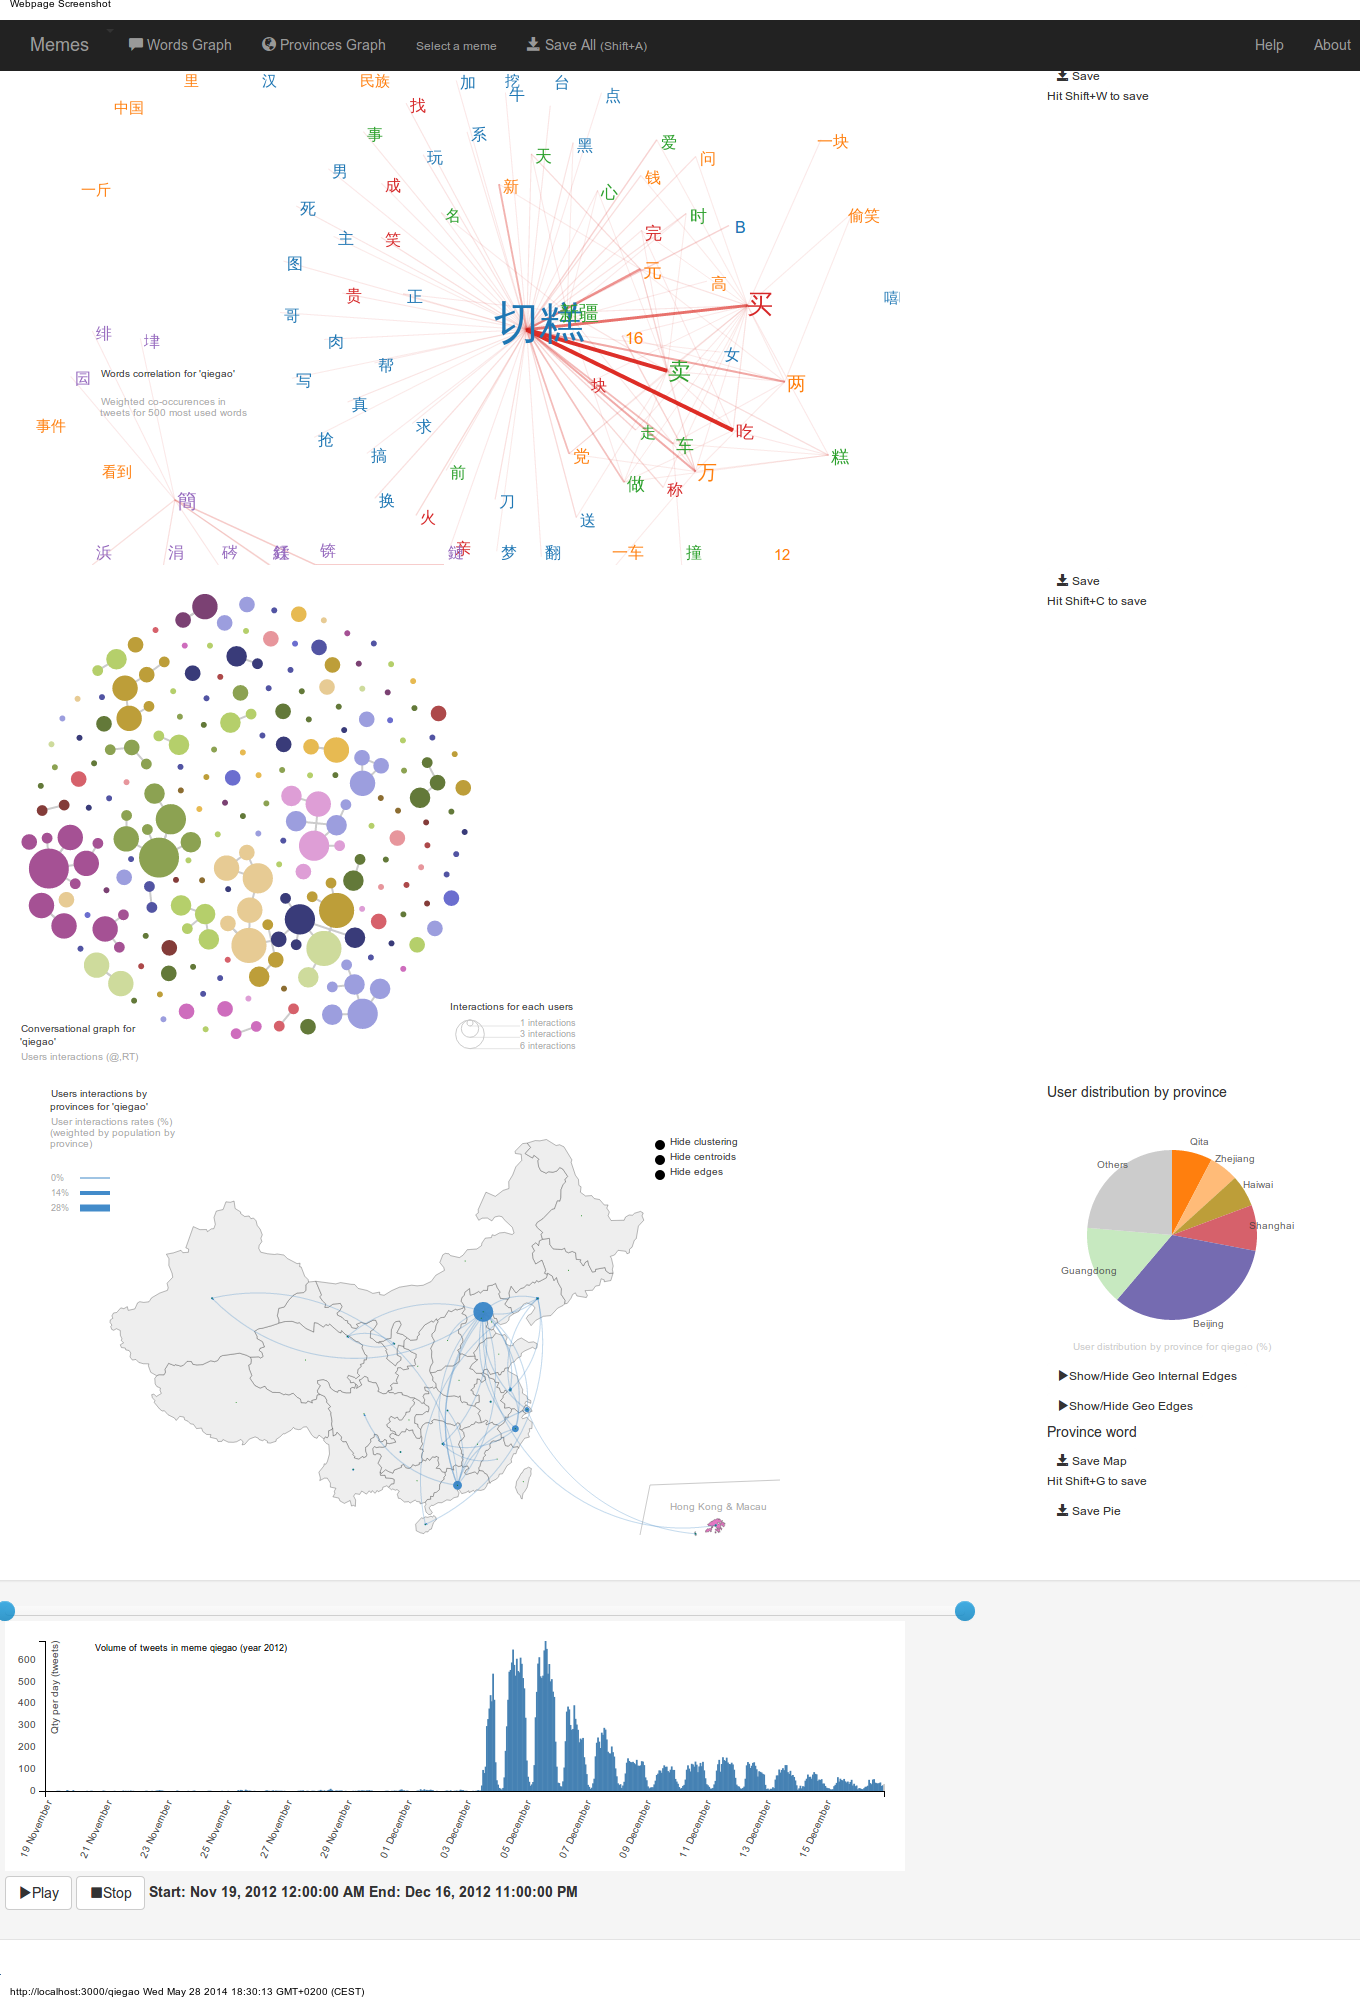
\includegraphics[width=6.7213in,height=8.3894in]{figures/chap3/chapitre3-img21.png}
    \caption{Interface d'exploration et de visualisation des données}
\end{figure}


\subsection[Validité et validation de l outil]{Validité et validation de l outil}

validité interne/externe (Tannery)